\begin{center}
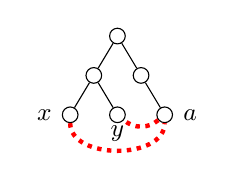
\begin{tikzpicture}[scale=.5,level distance=10mm, state/.style={circle, draw, minimum size=1mm}]]
  \tikzstyle{every node}=[font=\small, draw=black,circle,inner sep=2pt, minimum size=1mm]
  \tikzstyle{level 1}=[sibling distance=12mm, set style={{every node}+=[draw=black]}]
  \tikzstyle{level 2}=[sibling distance=12mm, set style={{every node}+=[draw=black]}]
  \tikzstyle{level 3}=[sibling distance=12mm,  set style={{every node}+=[draw=black]}]

    \node {}
     child {
        node {}
              child {node [label=left:{$x$}] (x) {}}
                child {node [label={[label distance=-1mm]below:{$y$}}] (y) {}}}
            child{ node {}
            child[fill=none] {edge from parent[draw=none]}
            child{node[label=right:{$a$}] (a) {}}};
    
    \draw[-,dotted,ultra thick,relative,red] (x) to[out=270,in=270] (a);
    
    \draw[-,dotted,ultra thick,relative,red] (a) to[out=40,in=-220] (y);
       
\end{tikzpicture}
\end{center}